La forma es uno de los factores fundamentales para reconocer un objeto. Es fácil reconocer en la figura \ref{delfin} a un delfín. Todo esto sin utilizar otros indicadores fundamentales como pueden ser el color o la textura del objeto, sin contar información adicional como el escenario de la imagen. Esto hace pensar que la forma contiene información valiosa para obtener buenos descriptores de las imágenes y por tanto pueden ser de utilidad para la recuperación de imágenes.\\


\begin{figure}[H]
\begin{center}

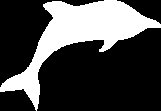
\includegraphics[width=0.3\textwidth]{img/delfin.jpg}
\end{center}

\caption{Silueta de un delfín.}
\label{delfin}
\end{figure}

Así pues, en este capítulo, explicaremos de manera breve uno de los descriptores más utilizados para el estudio de las formas, la curvatura, y la investigación realizada para obtener otros descriptores más cercanos al lenguaje cotidiano, utilizando la lógica difusa. Se introduce además una sección para introducir los conceptos básicos de la lógica difusa.\\

Destacar que no se trata de resolver el problema completo. Se deja a un lado problemas de una entidad propia como el preprocesamiento de las imágenes o la segmentación. Se supone que tenemos imágenes que simplemente son una máscara, donde un 1 indica la presencia del objeto y un 0 su ausencia en un determinado píxel.